\section{Methods}\label{methods}

\subsection{Data Set: a physics overview}\label{sec:data}

The field of dynamic systems encompasses a broad discipline, and a discussion of such can be approached both with a physics or a purely mathematical scope. A general but simple description is that it is the study of how a system evolves over time. For our purposes and investigations, we shall focus on the mathematical aspects of it, as we are interested in a dynamical system as a solution for a differential equation, which we face as a time-series evolution. Nonetheless, we will make use of physics tools in order to devise better-predicting algorithms.

A dynamical system can be categorized based on how it develops over time, but also how this behavior is affected by initial conditions and other rules. Two canonical examples of dynamical systems which exhibit completely different time evolution properties are the Lorenz attractor and a stable spiral.

\subsubsection{Stable Spiral}\label{sec:spiral}

The dynamics of a stable spiral evolve in such a way that the system's trajectory converges to a fixed point while spiraling inward. These oscillations around the fixed point are gradually dampened until the system reaches a steady state at a fixed point.
Suppose we have a two-dimensional system of coupled differential equations of the form

\begin{align}
    \frac{dx}{dt} &= ax + by \notag,\\
    \frac{dy}{dt} &= cx + dy.
    \label{eq:spiral}
\end{align}

The choice of $a,b,c,d \in \mathbb{R}$ completely determines the behavior of the solution, and for some of these values, albeit not all, the system is said to be a stable spiral. This condition is satisfied when the eigenvalues of the matrix formed by the coefficients are complex conjugates with a negative real part \cite{abell2022chapter6}. 

For illustration, \figref{fig:spiral} depicts the simulation of a stable spiral trajectory.

\begin{figure}[H]
\includegraphics[width= \linewidth]{figs/stable_spiral_a=0.2_b=1.0_c=1.0_d=0.2_plot.pdf}
    \caption{Trajectory of a simple stable spiral with coefficients $a = 0.2$, $b = -1.0$ , $c = 1.0$ , $d = 0.2$.}
    \label{fig:spiral}
\end{figure}


\subsubsection{Lorenz attractor}\label{sec:lorenz}

In contrast to the previous example, a Lorenz attractor presents some added complexity. Firstly, it is by definition a three-dimensional system, but more importantly, it exhibits what is called chaotic behavior \cite{hasselblatt2003first}. While there is no universal consensus on the definition of a chaotic system, all definitions agree chaotic systems are extremely sensitive to initial conditions. This means an arbitrary perturbation of such a set of conditions -or the current trajectory- will lead to vastly distinct asymptotic behavior.

The expression for the Lorenz attractor evolution consists of a set of three coupled nonlinear differential equations given by

\begin{align}
    \frac{dx}{dt} &= \sigma (y-x), \notag\\
    \frac{dy}{dt} &= x(\rho -z) - y, \notag\\
    \frac{dz}{dt} &= xy- \beta z.  
    \label{eq:lorenz}
\end{align}

For this problem, ${x,y,z}$ are the variables that determine the state of the system in the space while $\sigma, \rho$ and $\beta$ are, similarly to the constants $a,b,c,d$ of the stable spiral, parameters that influence largely how the system evolves. For illustration, \figref{fig:lorenz} depicts two particular Lorenz attractor trajectories.

\begin{figure}[H]
\includegraphics[width= \linewidth]{figs/lorenz.pdf}
    \caption{Simulation of two Lorenz attractor trajectories. While both are determined by \eqref{eq:lorenz}, they had two different initial conditions, hence the legend IC 1 and IC 2.}
    \label{fig:lorenz}
\end{figure}

\subsubsection{Generating the data}\label{sec:rk4}

Both of the above-mentioned systems are governed by differential equations, and as such, they can be solved numerically through some integration scheme such as forward-Euler or fourth-order Runge-Kutta. The latter was the algorithm of choice for the generated data sets.  

For our attractor, we will use the common choice of parameters $\sigma =10$, $\rho =28$, $\beta =8/3$. Although apparently arbitrary, this is a natural choice. Not only was it used by Lorenz himself \cite{lorenz1963deterministic}, but it generates complex and aesthetic trajectories that have been extensively investigated and benchmarked in the literature of numerical simulations. For the stable spiral, we used $a = 0.2$, $b = -1.0$, $c = 1.0$, $d = 0.2$ as it showed a good number of oscillations before reaching a steady state for our simulation time. 


\subsection{Feed-forward networks}
\begin{figure}[H]
\begin{center}
    

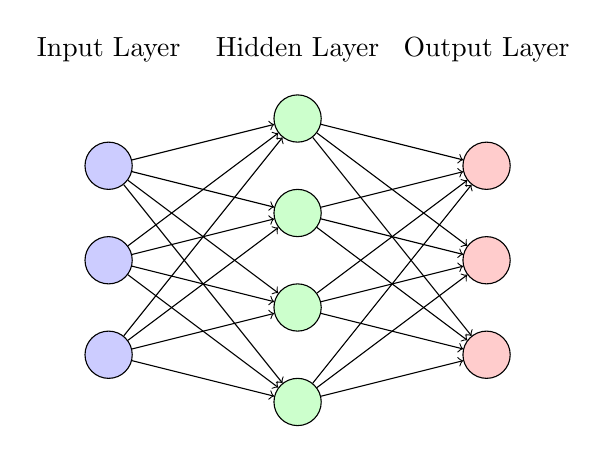
\begin{tikzpicture}[scale=1.2]
  % Input layer
  \foreach \i in {1,...,3}
    \node[circle, draw=black, fill=blue!20, minimum size=6mm] (input-\i) at (0,-\i) {};

  % Hidden layer
  \foreach \i in {1,...,4}
    \node[circle, draw=black, fill=green!20, minimum size=6mm] (hidden-\i) at (2,-\i+0.5) {};

  % Output layer
  \foreach \i in {1,...,3}
    \node[circle, draw=black, fill=red!20, minimum size=6mm] (output-\i) at (4,-\i) {};

  % Arrows
  \foreach \i in {1,...,3}
    \foreach \j in {1,...,4}
      \draw[->] (input-\i) -- (hidden-\j);

  \foreach \i in {1,...,4}
    \foreach \j in {1,...,3}
      \draw[->] (hidden-\i) -- (output-\j);

  % Labels
  \node[above] at (0,0) {Input Layer};
  \node[above] at (2,0) {Hidden Layer};
  \node[above] at (4,0) {Output Layer};
\end{tikzpicture}
\end{center}

    \caption{Basic schematic of a feed-forward neural network showing its layers and units.}
    \label{fig:ffn}
\end{figure}


In its general definition, a feed-forward neural network is a way to organize a set of function compositions in a sequential way. The algorithmic way of doing so is referred to as a network, given that it can be understood as being composed of individual but somehow connected units in a graph-like manner. 

The network is said to be of feed-forward type if information flows in one preferential direction in the network. This means each neuron receives inputs from the previous layer, and after multiplying it by a set of weights and adding some bias - and often composing it with some activation function - passes the result to neurons in the next layer. The way in which the units are organized in layers and how they are connected results in different architectures. 

The choice of the architecture of a network is often guided by the problem one aims at tackling, but most networks have some overlapping core structure in the form of input layers, hidden layers, output layers, and activation functions, as can be seen in \figref{fig:ffn}. The network's weights and biases are then iteratively updated via a gradient scheme that tries to converge to a global minimum of a cost-function. This cost function is a measurement of well the model performs, be it in regression, or classification problems.


\begin{align}
&            && \mathbf{h}_0 = \mathbf{x} \notag\\
&            && 
                \negthickspace% for compensation of rcases misalignment
                \begin{rcases}  
                \mathbf{a}_i= W_i * \mathbf{h}_{i-1} + \mathbf{b}_i \notag\\
                \mathbf{h}_i    = \sigma_i(\mathbf{a}_i) 
                    \end{rcases}&  i \in \{1, ..., L-1\}, \\
&            &&\mathbf{\hat{y}} = \sigma_L(W_y *\mathbf{h}_{L-1} + \mathbf{b}_y) 
\label{eq:FFN}
\end{align}

where $W_i$ and $b_i$ are respectively the weight matrix and bias vector of the i-th layer, $h_i$ represents the output of the i-th hidden layer and we are defining the 0-th hidden layer as the input of the network, $\mathbf{x}$. Similarly, $\sigma_i$ represents the activation function of each hidden layer and $L$ is the output layer. 

There are limitation of FFNNs, one of which being that FFNNs are not designed to handle sequential data (data for which the order matters) effectively because they lack the capabilities of storing information about previous inputs; each input is being treated independently. This is a limitation when dealing with sequential data where past information can be vital to correctly process current and future inputs.

\subsection{Recurrent networks}

In contrast to FFNs, recurrent networks introduce feedback connections, meaning the information is allowed to be carried to subsequent nodes across different time steps. These cyclic or feedback connections have the objective of providing the network with some kind of memory, making RNNs particularly suited for time-series data, natural language processing, speech recognition, and several other problems for which the order of the data is crucial. 

RNN architectures vary greatly in how they manage information flow and memory in the network. Different architectures often aim at improving some sub-optimal characteristics of the network. The simplest form of recurrent network, commonly called simple or vanilla RNN, for example, is known to suffer from the problem of vanishing gradients.
This problem arises due to the nature of backpropagation in time. Gradients of the cost/loss function may get exponentially small (or large) if there are many layers in the network, which is the case of RNN when the sequence gets long. Consequently, the convergence to correctly predicted values in the training process happens very slowly. This is particularly the case when using activation functions like the Sigmoid or hyperbolic tangent, (whose outputs are between 0 and 1 for Sigmoid, and -1 and 1 for $\tanh$), with equally small gradients by design ($<1$).

To address that, one natural alternative is to use the Long Short-Term Memory (LSTM) variation. While LSTMs are generally used, they also present the downside of being inefficient for large-scale models. For such problems, Gated recurrent units (GRUs) can be employed as they have a simpler architecture, thus being computationally faster. We will hereafter focus simply on the Vanilla and LSTM variants for their simplicity and popularity.

\subsubsection{Vanilla RNN}

The expression for the simplest Recurrent network resembles that of a regular feed-forward neural network of \eqref{eq:FFN}, but now with the concept of temporal dependencies as shown in the equations for the forward pass, \eqref{eq:rnn_forward},

\begin{align}
    \mathbf{a}^{(t)} & = U * \mathbf{x}^{(t)} + W * \mathbf{h}^{(t-1)} + \mathbf{b}, \notag \\
    \mathbf{h}^{(t)} &= \sigma_h(\mathbf{a}^{(t)}), \notag\\
    \mathbf{o}^{(t)} &= V * \mathbf{h}^{(t)} + \mathbf{c}, \notag\\
    \mathbf{\hat{y}}^{(t)} &= \sigma_y(\mathbf{o}^{(t)}).
    \label{eq:rnn_forward}
\end{align}

\onecolumngrid
\begin{center}

\begin{figure}
    \begin{adjustbox}{width=0.8\textwidth}
    \begin{tikzpicture}[item/.style={circle,draw,thick,align=center},
itemc/.style={item,on chain,join}]
 \begin{scope}[start chain=going right,nodes=itemc,every
 join/.style={-latex,very thick},local bounding box=chain]
 \path node (A0) {$h^{(0)}$} node (A1) {$h^{(1)}$} node (A2) {$h^{(2)}$} node[xshift=2em] (At)
 {$h^{(t)}$};
 \end{scope}
 \node[left=1em of chain,scale=2] (eq) {$=$};
 \node[left=2em of eq,item] (AL) {$h$};
 \path (AL.west) ++ (-1em,2em) coordinate (aux);
 \draw[very thick,-latex,rounded corners] (AL.east) -| ++ (1em,2em) -- (aux) 
 |- (AL.west);
 \foreach \X in {0,1,2,t} 
     {\draw[very thick,-latex] (A\X.north) -- ++ (0,2em)
     node[above,item,fill=gray!10] (h\X) {$\mathbf{o}^{(\X)}$};
     %\ifthenelse{\X!=t;}{ \path (A\X.east) -- ++ (1,1em) node[midway, above] {$W$};};
     \draw[very thick,latex-] (A\X.south) -- ++ (0,-2em)
     node[below,item,fill=gray!10] (x\X) {$\mathbf{x}^{(\X)}$};}
 \draw[white,line width=0.8ex] (AL.north) -- ++ (0,1.9em);
 \draw[very thick,-latex] (AL.north) -- ++ (0,2em)
 node[above,item,fill=gray!10] {$y$};

 \draw[very thick,latex-] (AL.south) -- ++ (0,-2em)
 node[below,item,fill=gray!10] {$\mathbf{x}$};
 \path (x2) -- (xt) node[midway,scale=2,font=\bfseries] {\dots};

\foreach \X in {0,1,2} 
    \path (A\X.east) -- ++ (1,1em) node[midway, above] {$W$};
\foreach \X in {0,1,2, t} 
    \path (A\X.north) -- ++ (1,1em) node[midway, above] {$V$};
\foreach \X in {0,1,2,t} 
    \path (A\X.south) -- ++ (1,0em) node[midway, below] {$U$};
\end{tikzpicture}
\end{adjustbox}
    \caption{Folded versus unfolded representation of a Vanilla RNN}
    \label{fig:rnn}
\end{figure}
\end{center}

\twocolumngrid

Equation \eqref{eq:rnn_forward},  can be better understood from the schematics of \figref{fig:rnn}. Here, the superscripts denote the temporal dependency of each pass. As usual, $\mathbf{h}$ represents the output of the hidden layer, after its activation $\sigma_h$, while $\mathbf{y}$ and $\sigma_y$ have the analogous role for the output layer. Similarly to a regular FFN, $\mathbf{b} $ and $\mathbf{c}$ represent the bias of the hidden layers and the output layers respectively. Notice however that we have weight matrices that modulate two inputs to a fixed hidden layer, $U$ and $W$. Indeed, hidden layers now receive a temporal input of the data $\mathbf{x}^{(t)}$ but also from the output of the same hidden layer in a previous temporal step, $\mathbf{h}^{(t-1)}$. Finally, the output layer's input is also modulated by weights $V$.

For this breakdown of equation \eqref{eq:rnn_forward} it is important to note that we are not specifying which layer of the network we are propagating, to avoid carrying indices. As can be seen from \figref{fig:rnn}, RNNs are often depicted in both a folded and an unfolded visualization, but it is important to note that a unit $h^{(t)}$ can be composed of many layers.

The learning procedure for RNNs also follows the same idea as that of regular FFNs: we need to optimize weights and bias so that the loss function $\mathcal{L}$ which assesses how well the model performs, gets minimized. To construct $\mathcal{L}$, it is paramount it takes into account all the temporal outputs, $\mathbf{y}^{(t)}$, and sum over their respective losses,

\begin{align}
    \mathcal{L}= \sum_t L^{(t)}.
    \label{eq:loss_rnn}
\end{align}

The choice of the individual losses $L^{(t)}$ is heavily dependent on the problem at hand, and shall be discussed in the following section \ref{sec:loss_funct}. This temporal dependency of the loss means the usual back-propagation process to evaluate the gradient of the parameters and update them depends on previous time steps due to the chain rule. For that reason, it is called back-propagation through time (BPTT), but the idea behind it is the same as for regular back-propagation: derive the loss function with respect to the parameters.

\subsubsection{Backpropagation through time}

The subsequent derivation follows closely the explanations of \cite{Goodfellow}, however, we shall not assume any loss function for now. To derive the expression of the gradients of $\mathcal{L}$ for the RNN, we need to start recursively from the nodes closer to the output layer in the temporal unrolling scheme - such as $\mathbf{o}$ and $\mathbf{h}$ at final time $t = \tau$,

\begin{align}
    (\nabla_{ \mathbf{o}^{(t)}} \mathcal{L})_{i} &= \frac{\partial \mathcal{L}}{\partial L^{(t)}}\frac{\partial L^{(t)}}{\partial o_{i}^{(t)}}, \notag\\
    \nabla_{\mathbf{h}^{(\tau)}} \mathcal{L} &= \mathbf{V}^\mathsf{T}\nabla_{ \mathbf{o}^{(\tau)}} \mathcal{L}.
    \label{eq:rnn_gradients1}
\end{align}

For the following hidden nodes, we have to iterate through time, so by the chain rule, 

\begin{align}
    \nabla_{\mathbf{h}^{(t)}} \mathcal{L} &= \left(\frac{\partial\mathbf{h}^{(t+1)}}{\partial\mathbf{h}^{(t)}}\right)^\mathsf{T}\nabla_{\mathbf{h}^{(t+1)}}\mathcal{L} + \left(\frac{\partial\mathbf{o}^{(t)}}{\partial\mathbf{h}^{(t)}}\right)^\mathsf{T}\nabla_{ \mathbf{o}^{(t)}} \mathcal{L}.
    \label{eq:rnn_gradients2}
\end{align}

Similarly, the gradients of $\mathcal{L}$ with respect to the weights and biases follow,

\begin{align}
    \nabla_{\mathbf{c}} \mathcal{L} &=\sum_{t}\left(\frac{\partial \mathbf{o}^{(t)}}{\partial \mathbf{c}}\right)^\mathsf{T} \nabla_{\mathbf{o}^{(t)}} \mathcal{L} \notag\\
    \nabla_{\mathbf{b}} \mathcal{L} &=\sum_{t}\left(\frac{\partial \mathbf{h}^{(t)}}{\partial \mathbf{b}}\right)^\mathsf{T}        \nabla_{\mathbf{h}^{(t)}} \mathcal{L} \notag\\
    \nabla_{\mathbf{V}} \mathcal{L} &=\sum_{t}\sum_{i}\left(\frac{\partial \mathcal{L}}{\partial o_i^{(t)} }\right)\nabla_{\mathbf{V}^{(t)}}o_i^{(t)} \notag\\
    \nabla_{\mathbf{W}} \mathcal{L} &=\sum_{t}\sum_{i}\left(\frac{\partial \mathcal{L}}{\partial h_i^{(t)}}\right)\nabla_{\mathbf{w}^{(t)}} h_i^{(t)} \notag\\
    \nabla_{\mathbf{U}} \mathcal{L} &=\sum_{t}\sum_{i}\left(\frac{\partial \mathcal{L}}{\partial h_i^{(t)}}\right)\nabla_{\mathbf{U}^{(t)}}h_i^{(t)}.
    \label{eq:rnn_gradients3}
\end{align}


The pseudo-code in \ref{algo:bptt} illustrates algorithmically how information and the gradients flow in a vanilla RNN based on the previous equations of \eqref{eq:rnn_gradients1}, \eqref{eq:rnn_gradients2} and \eqref{eq:rnn_gradients3}. Note that it already assumes the bias and weights to be initialized - for such, it is usual to use normal random distribution $\mathcal{N}(0, \sigma)$, where $\sigma$ is small to prevent exploding gradients.

\begin{figure}
    \begin{algorithm}[H]
    \caption{ Single Vanilla RNN epoch}
    \label{algo:bptt}
        \begin{algorithmic}
            \State $\boldsymbol{\delta_h},\boldsymbol{\delta_W},\boldsymbol{\delta_V},\boldsymbol{\delta_b},\boldsymbol{\delta_c}  = \mathbf{0}$ \Comment{Initialize gradient accumulation states}
            \For {each time step $t$ in the sequence}
                \State $\mathbf{o}^{(t)}$, $\mathbf{h}^{(t)}$ $\leftarrow$ \textbf{Forward pass}
            \EndFor
            \State $\mathcal{L}\leftarrow$ \textbf{Compute loss} 
            \State \textbf{Compute gradient of output layer:}
            \State $(\nabla_{ \mathbf{o}^{(t)}} \mathcal{L})_{i} $ \Comment{Based on specific loss}
            \State \textbf{Compute gradient of hidden layer at $t = \tau$:}
            \State $\boldsymbol{\delta_h} \leftarrow \nabla_{\mathbf{h}^{(\tau)}} \mathcal{L} $ 
            \State \textbf{Backpropagate through time:}
            \For {each time step $t = \tau - 1$ to $t=1$}
                \State \textbf{Compute and update hidden state gradient:}
                \State $\boldsymbol{\delta_h} = \left(\frac{\partial\mathbf{h}^{(t+1)}}{\partial\mathbf{h}^{(t)}}\right)^\mathsf{T}\boldsymbol{\delta_h} + \left(\frac{\partial\mathbf{o}^{(t)}}{\partial\mathbf{h}^{(t)}}\right)^\mathsf{T}\nabla_{ \mathbf{o}^{(t)}} \mathcal{L}$ 

                \State \textbf{Acumulate parameter gradients:}
                \State $\boldsymbol{\delta_c} += \left(\frac{\partial \mathbf{o}^{(t)}}{\partial\mathbf{c}}\right)^\mathsf{T}\nabla_{\mathbf{o}^{(t)}} \mathcal{L}$
                \State $\boldsymbol{\delta_b} += \left(\frac{\partial \mathbf{h}^{(t)}}{\partial\mathbf{b}}\right)^\mathsf{T}\nabla_{\mathbf{h}^{(t)}} \mathcal{L}$
                \State $\boldsymbol{\delta_V} +=\sum_{i} \left(\frac{\partial \mathcal{L}}{\partial o_{i}^{(t)}}\right)\nabla_{\mathbf{V}^{(t)}}o^{(t)}_{i}$
                \State $\boldsymbol{\delta_W} +=\sum_{i} \left( {\delta_{\mathbf{h}}}\right)_i\nabla_{\mathbf{W}^{(t)}}h^{(t)}_{i}$
                \State $\boldsymbol{\delta_U} +=\sum_{i} \left( {\delta_{\mathbf{h}}}\right)_i\nabla_{\mathbf{U}^{(t)}}h^{(t)}_{i}$
            \EndFor
            \State \textbf{Weight and bias update:}
            \State $\enspace \{W, U, V, \mathbf{b}, \mathbf{c} \}-= \alpha \cdot  \{\boldsymbol{\delta_W} , \boldsymbol{\delta_U} , \boldsymbol{\delta_V} , \boldsymbol{\delta_b} ,\boldsymbol{\delta_c} \}$
        \end{algorithmic}
    \end{algorithm}
    \caption*{Pseudo code for the forward and backward propagations of a simple RNN. Equations for the gradient expressions follow \eqref{eq:rnn_gradients1}, \eqref{eq:rnn_gradients2}, \eqref{eq:rnn_gradients3}}
\end{figure}


\subsubsection{LSTM}
The Long Short Term Memory RNN is a type of RNN designed to avoid the vanishing or exploding gradient caused easily by the Vanilla RNN, which makes it difficult to learn long-range dependencies in a sequence.  Given the recurrent relation in equation \eqref{eq:rnn_gradients2}, the long-term gradient can end up having many factors of $\partial \mathbf{h}^{(t+1)}/\partial\mathbf{h}^{(t)}$, which may be close to zero or excessively large, leading to vanishing or exploding gradients respectively. In 1997, in order to address the aforementioned problem, Hochreiter and Schmidhuber introduced LSTM which truncates the gradient where it does not incur significant detriment to performance \cite{Hochreiter97}.

The LSTM is a unit cell that is made of three gates: the input gate, the forget gate, and the output gate. It also introduces a cell state $c$, which can be thought of as the long-term memory, and a hidden state $h$ which can be thought of as the short-term memory. As illustrated in Figure~\ref{fig:lstm}. \\
The first stage is called the forget gate, where we combine the input at (say, time $t$), and the hidden cell state input at $t-1$, passing it through the Sigmoid activation function and then performing an element-wise multiplication, denoted by $\otimes$.
It follows 
\[\mathbf{f}^{(t)} = \sigma(W_f\mathbf{x}^{(t)} + U_f\mathbf{h}^{(t-1)} + \mathbf{b}_f) \]
where $W$ and $U$ are the weights respectively.
This is called the forget gate since the Sigmoid activation function's outputs are very close to $0$ if the argument for the function is very negative, and $1$ if the argument is very positive. Hence we can control the amount of information we want to take from the long-term memory.\\

The next stage is the input gate, which consists of both a Sigmoid function ($\sigma_i$), which decide what percentage of the input will be stored in the long-term memory, and the $\tanh_i$ function, which decide what is the full memory that can be stored in the long term memory. When these results are calculated and multiplied together, it is added to the cell state or stored in the long-term memory, denoted as $\oplus$. \\
It follows
\[\mathbf{i}^{(t)} = \sigma_g(W_i\mathbf{x}^{(t)} + U_i\mathbf{h}^{(t-1)} + \mathbf{b}_i),\]
\[\mathbf{\tilde{c}}^{(t)} = \tanh(W_c\mathbf{x}^{(t)} + U_c\mathbf{h}^{(t-1)} + \mathbf{b}_c),\] again the $W$ and $U$ are the weights.

The forget gate and the input gate together also update the cell state with the following equation, 
\[\mathbf{c}^{(t)} = \mathbf{f}^{(t)} \otimes \mathbf{c}^{(t-1)} + \mathbf{i}^{(t)} \otimes \mathbf{\tilde{c}}^{(t)},\] where $f^{(t)}$ and $i^{(t)}$ are the outputs of the forget gate and the input gate, respectively.

The final stage of the LSTM is the output gate, and  its purpose is to update the short-term memory.  To achieve this, we take the newly generated long-term memory and process it through a hyperbolic tangent ($\tanh$) function creating a potential new short-term memory. We then multiply this potential memory by the output of the Sigmoid function ($\sigma_o$). This multiplication generates the final output as well as the input for the next hidden cell ($h^{\langle t \rangle}$) within the LSTM cell.


It follows,
\[\begin{aligned}
\mathbf{o}^{(t)} &= \sigma_g(W_o\mathbf{x}^{(t)} + U_o\mathbf{h}^{(t-1)} + \mathbf{b}_o), \\
\mathbf{h}^{(t)} &= \mathbf{o}^{(t)} \otimes \sigma_h(\mathbf{c}^{(t)}). \\
\end{aligned}\]
where $\mathbf{W_o,U_o}$ are the weights of the output gate and $\mathbf{b_o}$ is the bias of the output gate.

\begin{figure}
    \centering
    
\newcommand{\empt}[2]{$#1^{\langle #2 \rangle}$}

\begin{tikzpicture}[scale=0.95,
    % GLOBAL CFG
    font=\sf \scriptsize,
    >=LaTeX,
    % Styles
    cell/.style={% For the main box
        rectangle, 
        rounded corners=5mm, 
        draw,
        very thick,
        },
    operator/.style={%For operators like +  and  x
        circle,
        draw,
        inner sep=-0.5pt,
        minimum height =.2cm,
        },
    function/.style={%For functions
        ellipse,
        draw,
        inner sep=1pt
        },
    ct/.style={% For external inputs and outputs
        circle,
        draw,
        line width = .75pt,
        minimum width=1cm,
        inner sep=1pt,
        },
    gt/.style={% For internal inputs
        rectangle,
        draw,
        minimum width=4mm,
        minimum height=3mm,
        inner sep=1pt
        },
    mylabel/.style={% something new that I have learned
        font=\scriptsize\sffamily
        },
    ArrowC1/.style={% Arrows with rounded corners
        rounded corners=.25cm,
        thick,
        },
    ArrowC2/.style={% Arrows with big rounded corners
        rounded corners=.5cm,
        thick,
        },
    ]

%Start drawing the thing...    
    % Draw the cell: 
    \node [cell, minimum height =4cm, minimum width=6cm] at (0,0){} ;

    % Draw inputs named ibox#
    \node [gt] (ibox1) at (-2,-0.75) {$\sigma_f$};
    \node [gt] (ibox2) at (-1.5,-0.75) {$\sigma_i$};
    \node [gt, minimum width=1cm] (ibox3) at (-0.5,-0.75) {$\tanh_i$};
    \node [gt] (ibox4) at (0.5,-0.75) {$\sigma_o$};

   % Draw opérators   named mux# , add# and func#
    \node [operator] (mux1) at (-2,1.5) {$\times$};
    \node [operator] (add1) at (-0.5,1.5) {+};
    \node [operator] (mux2) at (-0.5,0) {$\times$};
    \node [operator] (mux3) at (1.5,0) {$\times$};
    \node [function] (func1) at (1.5,0.75) {$\tanh_o$};

    % Draw External inputs? named as basis c,h,x
    \node[ct, label={[mylabel]Cell}] (c) at (-4,1.5) {\empt{c}{t-1}};
    \node[ct, label={[mylabel]Hidden}] (h) at (-4,-1.5) {\empt{h}{t-1}};
    \node[ct, label={[mylabel]left:Input}] (x) at (-2.5,-3) {\empt{x}{t}};

    % Draw External outputs? named as basis c2,h2,x2
    \node[ct, label={[mylabel]Next Cell}] (c2) at (4,1.5) {\empt{c}{t}};
    \node[ct, label={[mylabel]Next Hidden}] (h2) at (4,-1.5) {\empt{h}{t}};
    \node[ct, label={[mylabel]left:Output}] (x2) at (2.5,3) {\empt{h}{t}};

% Start connecting all.
    %Intersections and displacements are used. 
    % Drawing arrows    
    \draw [ArrowC1] (c) -- (mux1) -- (add1) -- (c2);

    % Inputs
    \draw [ArrowC2] (h) -| (ibox4);
    \draw [ArrowC1] (h -| ibox1)++(-0.5,0) -| (ibox1); 
    \draw [ArrowC1] (h -| ibox2)++(-0.5,0) -| (ibox2);
    \draw [ArrowC1] (h -| ibox3)++(-0.5,0) -| (ibox3);
    \draw [ArrowC1] (x) -- (x |- h)-| (ibox3);

    % Internal
    \draw [->, ArrowC2] (ibox1) -- (mux1);
    \draw [->, ArrowC2] (ibox2) |- (mux2);
    \draw [->, ArrowC2] (ibox3) -- (mux2);
    \draw [->, ArrowC2] (ibox4) |- (mux3);
    \draw [->, ArrowC2] (mux2) -- (add1);
    \draw [->, ArrowC1] (add1 -| func1)++(-0.5,0) -| (func1);
    \draw [->, ArrowC2] (func1) -- (mux3);

    %Outputs
    \draw [-, ArrowC2] (mux3) |- (h2);
    \draw (c2 -| x2) ++(0,-0.1) coordinate (i1);
    \draw [-, ArrowC2] (h2 -| x2)++(-0.5,0) -| (i1);
    \draw [-, ArrowC2] (i1)++(0,0.2) -- (x2);

\end{tikzpicture}

\caption{LSTM illustration \footnote{source: https://tex.stackexchange.com/questions/432312/how-do-i-draw-an-lstm-cell-in-tikz}}
    \label{fig:lstm}
\end{figure}


\subsubsection{Training and testing trajectories}

Training and testing procedures in recurrent neural networks follow what is usual for regular FNNs, but some special consideration needs to be taken into account due to the sequential character of the data. Training and testing batches must not be randomly shuffled for it would clearly decorrelate the time-series points and leak future information into present or past points of the model. 

Additionally, the training algorithm in Algorithm (\ref{algo:bptt}) can become computationally costly, especially if the losses are evaluated for all previous time steps. While other architectures such as that of GRUs can be used to mitigate that, it is also possible to introduce another hyperparameter responsible for controlling how much of the network will be unfolded in the training process, adjusting how much the network will remember from previous points in time. We called this parameter the \emph{look-back}. Similarly, the number of steps the network predicts in the future per iteration greatly influences the assessment of the loss function. we called this parameter the \emph{look-ahead}.

The training and testing batches were separated into whole trajectories. This means that instead of training and testing on different fractions of the same trajectory, all trajectories that were tested had completely new initial conditions. In this sense, from a total of 10 initial conditions (independent trajectories), 9 were used for training and 1 for testing. Each trajectory consisted of 800 points in each space coordinate.

\subsection{On the choice of the loss function}  \label{sec:loss_funct}

Our problem is essentially a time-series forecasting problem, so, we are free to choose the loss function amongst the big collection of regression losses. Using the mean-squared error of the predicted versus factual trajectories of the dynamic systems is a natural choice for it is a way to measure their discrepancy in space, and it punished outliers strongly for its quadratic form. Furthermore, it is a convex function, so given sufficient time and appropriate learning rates, it is guaranteed to converge to global minima irrespective of the weight's random initialization. For completeness' sake, the expression for this loss function can be written 

\begin{align}
    \mathcal{L}_{MSE} = \frac{1}{N}\sum_{i}^N (y(\mathbf{x}_i) - \hat{y}(\mathbf{x}_i, \mathbf{\theta}))^2
    \label{eq:mse_loss}
\end{align}

where we are denoting $\mathbf{\theta}$ as the set of all parameters of the network, and $\mathbf{x}_i$ is our input. 

\subsubsection{The "naivety" of data-driven losses}

Simply using a loss function that is based on the observational and predicted data, such as the one in equation \eqref{eq:mse_loss} is commonly referred to as a purely data-driven approach. While this is a well-established way of assessing regressions, it does not make use of other intuitions we might have over the problem we are trying to solve. At the same time, it is a well-established fact that neural network models are data-greedy - they need large amounts of data to be able to generalize predictions outside the training set. One way to try to mitigate this is by using  physics-informed neural networks (PINNs) when possible.

Trying to improve the performance of our model beyond training sets, PINNs then add physics-informed penalties to the loss function. In essence, this means that we add a worse evaluation score to predictions that do not respect physical laws we think our real data should obey. This procedure often has the advantage of trimming the parameter space without adding bias to the model if the constraints imposed are correct, but the choice of the physical laws can be a delicate one. 


\subsubsection{Adding physics to the loss function}

A general way of expressing this added penalty to the loss function is shown in \eqref{eq:custom_loss} below,

\begin{align}
    \mathcal{L} = w_{MSE}\mathcal{L}_{MSE} + w_{PI}\mathcal{L}_{PI}.
    \label{eq:custom_loss}
\end{align}

Here, the weights $w_{MSE}$ and $w_{PI}$ explicitly mediate how much influence the specific parts of the total loss function should contribute. In our experimentations with the additional physics penalty, we limited results to only have $w_{MSE} = 1.0$ and $w_{PI}= 0.5$.

For one, it is important to note that this procedure is not a universal strategy to predict time-series data. In a general sense, the system need not obey the laws of physics. For instance, the Lorenz attractor, given its attractor behavior, does not conserve momentum.

While we are working with RNNs, the general schematics behind PINNs is illustrated in \figref{fig:PINNs} using a feed-forward net. The standard approach to construct $\mathcal{L}_{PI}$ is to ensure the outputs of the network satisfies the differential equations at hand. The outputs of the NN are often differentiated via an automatic differentiation software such as JAX \cite{jax2018github}. In our case, a natural approach would be

\begin{align}
    \mathcal{L}_{PI} &=     \frac{d \hat{x}}{dt} - \sigma (\hat{y}-\hat{x}) \notag\\
    & + \frac{d\hat{y}}{dt} - \hat{x}(\rho -\hat{z}) - \hat{y} \notag\\
    & +\frac{d\hat{z}}{dt} - \hat{x}\hat{y}- \beta \hat{z},
\end{align}

where we denoted with hats the neural network outputs. As long as the dynamics of the predictions respect the differential equations, this loss will be minimized. However, since we are working with recurrent neural networks that output one predicted time-step at a time during the training process, taking the derivative in time would not be straightforward. For this reason, we approach the problem of adding physics to the RNN in a similar but subtly different way. 

\begin{figure}[H]
\begin{center}
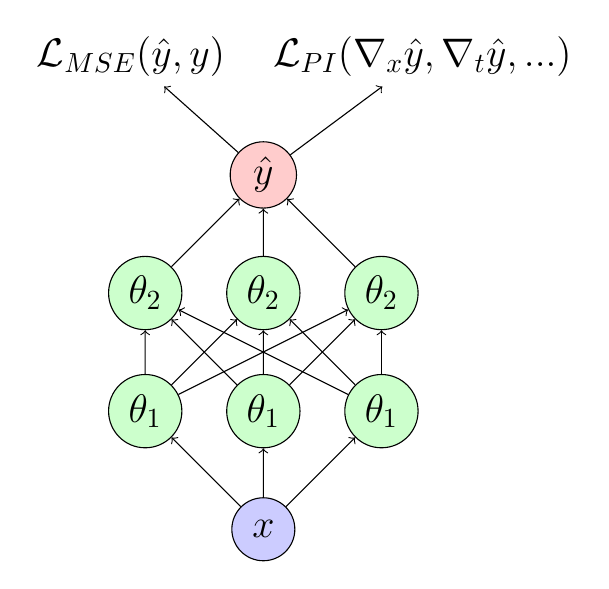
\begin{tikzpicture}[scale=1.5]
  % Input layer
  \foreach \i in {1}
    \node[circle, draw=black, fill=blue!20, minimum size=8mm] (input-\i) at (-\i, 0) {\Large $x$};

  % Hidden layer
  \foreach \i in {1,...,3}
    \node[circle, draw=black, fill=green!20, minimum size=8mm] (hidden1-\i) at (-\i+1, 1) {\Large
 $\theta_{1} $};

  \foreach \i in {1,...,3}
    \node[circle, draw=black, fill=green!20, minimum size=8mm] (hidden2-\i) at (-\i+1, 2) {\Large
 $\theta_{2} $};

  % Output layer
  \foreach \i in {1}
    \node[circle, draw=black, fill=red!20, minimum size=8mm] (output-\i) at (-\i , 3 ) {\Large $\hat{y}$};

 % eq layer
  \foreach \i in {1}
    \node[right] (equation1-\i) at (-\i, 4) {\Large
 $\mathcal{L}_{PI}(\nabla_x \hat{y},  \nabla_t \hat{y}, ...)$};

   \foreach \i in {1}
    \node[right] (equation2-\i) at (-\i - 2, 4) {\Large
 $\mathcal{L}_{MSE}(\hat{y}, y)$};


  % Arrows
  \foreach \i in {1}
    \foreach \j in {1,...,3}
      \draw[->] (input-\i) -- (hidden1-\j);
    
  \foreach \i in {1,...,3}
    \foreach \j in {1,...,3}
      \draw[->] (hidden1-\i) -- (hidden2-\j);

  \foreach \i in {1,...,3}
    \foreach \j in {1}
      \draw[->] (hidden2-\i) -- (output-\j);

    \draw[->](output-1) -- (equation1-1);
    \draw[->](output-1) -- (equation2-1);

\end{tikzpicture}
\end{center}
\caption{Sketch of the concurrent assessment of both physics-informed and data-driven losses.}
\label{fig:PINNs}
\end{figure}


As mentioned, the Lorenz attractor does not conserve momentum. Therefore, we cannot simply add a penalty term for when the subsequent temporal values of the right-hand side (RHS) of the differential equations (DE) (\ref{eq:lorenz}) differ from the initial one. To still enforce learning of the differential equation we instead construct the RHS of the DE from the positions predictions during training. We then compare those values with the same RHS of the DEs given the true trajectories. More specifically, the added physics loss was given by

\begin{align}
    \mathcal{L}_{PI} &=    MSE(\sigma (y-x), \sigma (\hat{y}-\hat{x})) \notag \\
    & + MSE(x(\rho -z) - y , \hat{x}(\rho -\hat{z}) - \hat{y}) \notag \\
    & +MSE(xy- \beta z , \hat{x}\hat{y}- \beta \hat{z})
\end{align}

The physics-informed term in the custom loss function represents the difference between the predicted derivatives of the Lorenz system and the true derivatives, as defined by the Lorenz equations. In other words, it measures how well the predicted trajectories of the system obey the physical laws that govern the Lorenz system.

By incorporating this physics-informed term into the loss function, the LSTM is encouraged to generate predictions that are not only accurate but also physically meaningful. This is important because the Lorenz system is a highly nonlinear and chaotic system, and therefore making predictions, especially long ones, is a hard task.